\subsection{RQ4: Characteristics of answer pattern of new languages}
\label{RQ3}
In Stack Overflow, the community size and age of a language are most likely to influence the answer interval. With time, the answer interval is likely to be decreased. To observe the anticipated change in intervals of new languages, we extracted several features from Stack Overflow like frequency of questions, questions without having any answer (no answer), questions having an accepted answer (accepted answer) and questions without an accepted answer (no accepted answer). An insight into the evolution of new languages is presented in Figure~\ref{fig:Evolution of new languages}.

\begin{figure}[htbp]

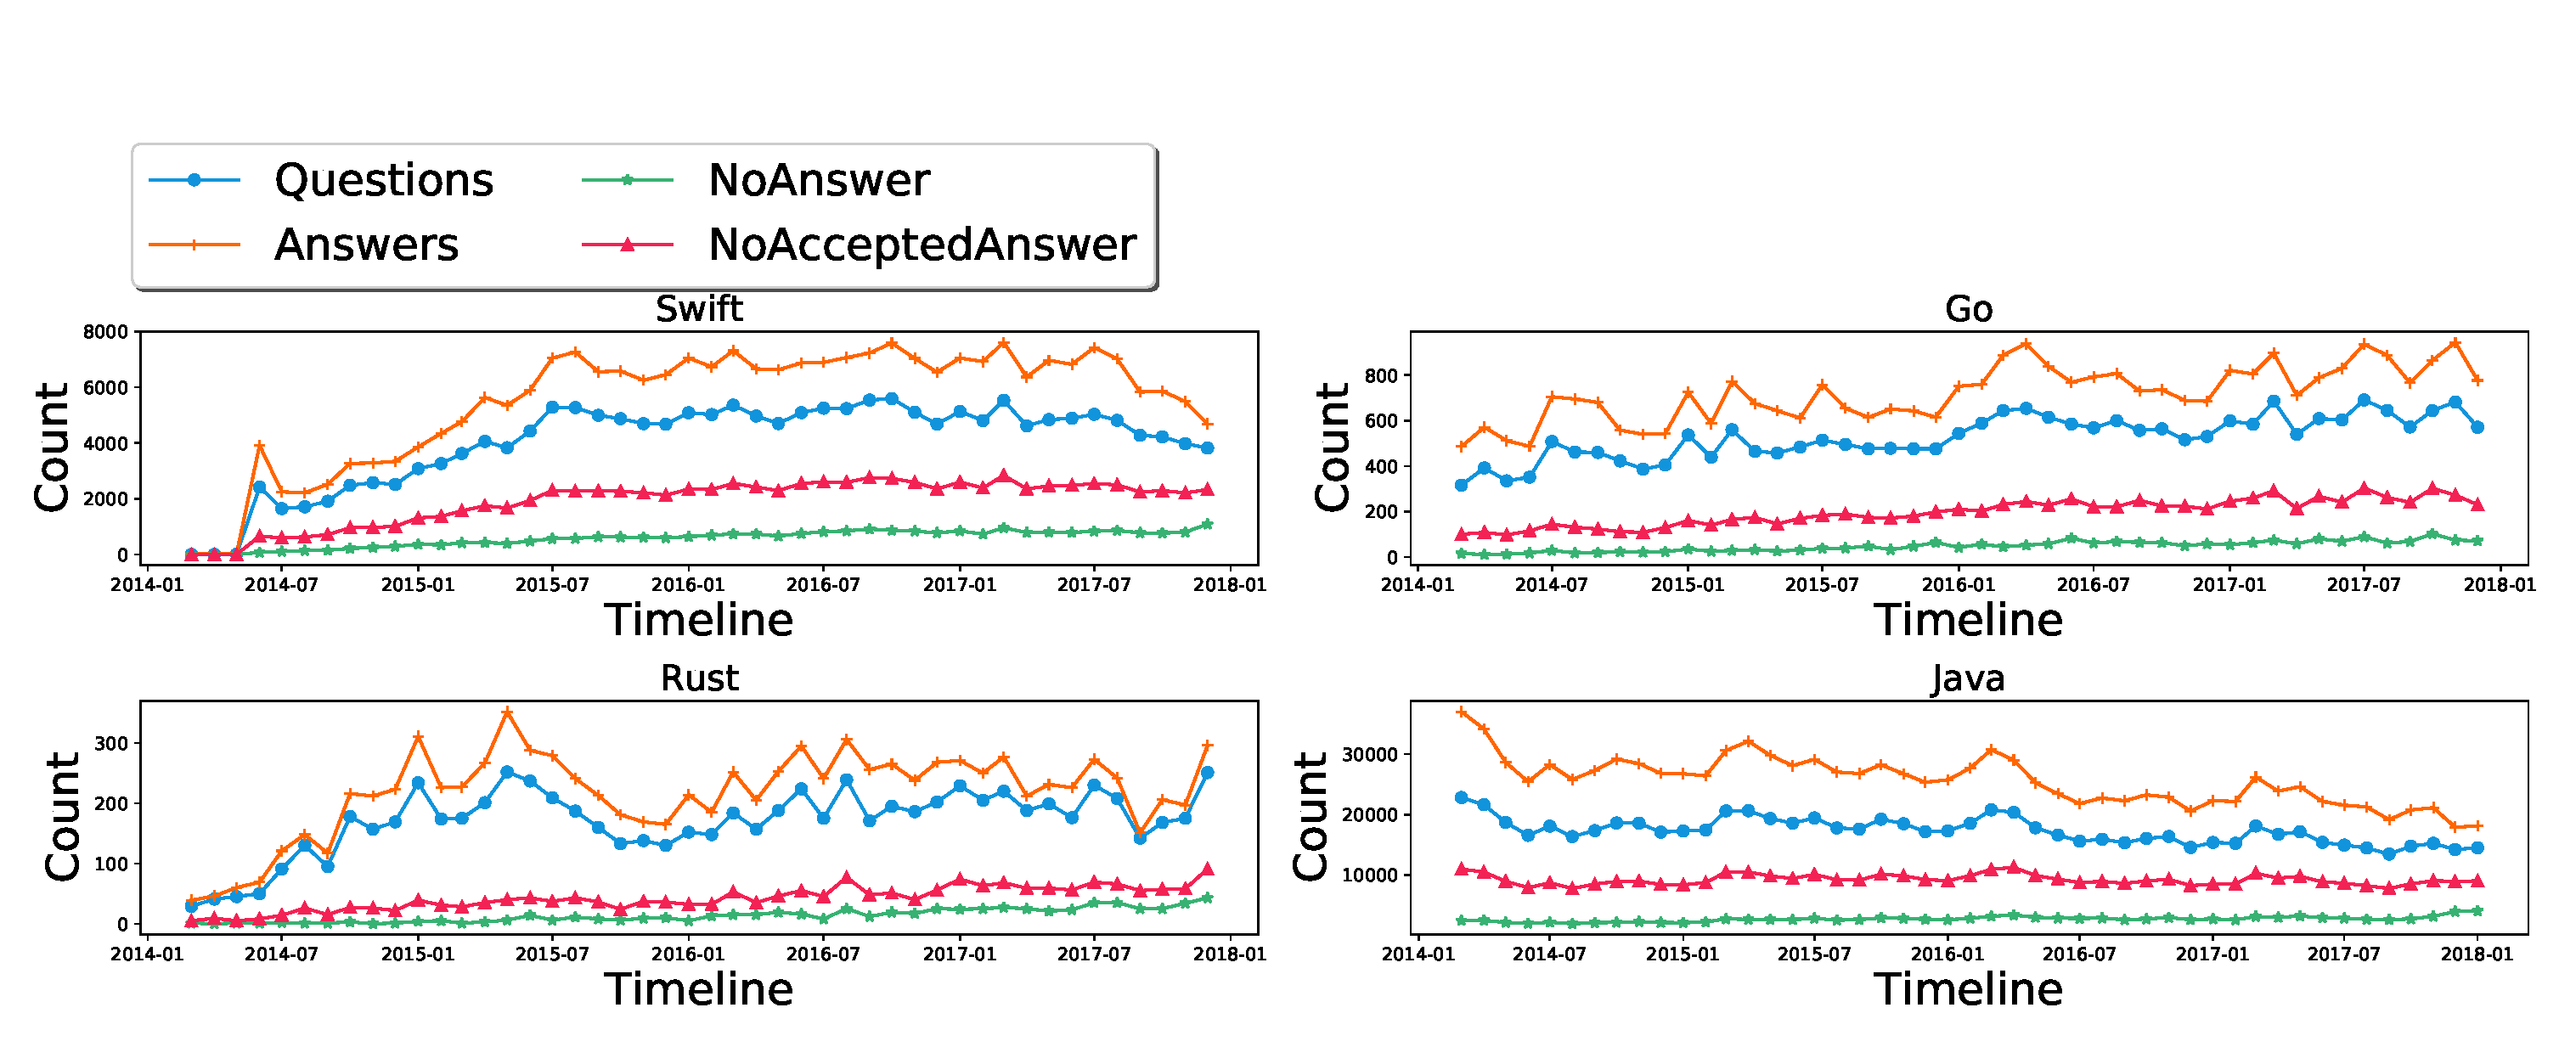
\includegraphics[scale=0.28]{figures/Evolution.eps} 
\caption{Question, No answer, Accepted answer, and No accepted answer count of languages in Stack Overflow}
\label{fig:Evolution of new languages}
\end{figure}

\iffalse
It is prominent in Figure~\ref{fig:Evolution of new languages} that the question count curve of Swift language (Figure~\ref{fig:Attributes of Swift Language}) is much smoother than the other two languages. The reason of smoothness is related to the closed issue ratio. Earlier, we have described the two states of GitHub issue. Based on the two states, we defined the closed issue ratio as,

\begin{equation}
{Closed \quad issue \quad ratio=}
\left[\dfrac{Closed\quad issue}
{Closed\quad issue+Open\quad issue}\right]
\label{eq:Closed Issue Ratio}
\end{equation}

We can say that the closed issue ratio means how much problems have been solved. It can be used as a measure of an active development team. Closed issue ratio one means all problems that were raised in that month were solved. We collected all the issue of the official repositories of new languages and calculated closed issue ratio,

\begin{table}[]
%\centering

\begin{tabular}{|l|l|l|l|}
\hline
 Language& Mean& Variance& Median\\ \hline
 Swift &  0.984  & 0.001 & 0.993 \\ \hline
 Go    &  0.901  & 0.01  & 0.917 \\ \hline
 Rust  &  0.95   & 0.006 & 0.984 \\ \hline

\end{tabular}%

\caption{Statistics of the closed issue ratio of new  languages.}
\label{table:Issue ratio}
\end{table}
From Table~\ref{table:Issue ratio}, we can say Swift has a very active development team with the closed issue ratio close to one. Maybe that is why the question frequency for Swift is smoother than the other two languages.
\fi

Based on the release date of new languages, we have defined two states for languages (1) Evolving state: the language has just been released, it lacks experts and other resources in Stack Overflow, and (2) Matured State: the language has a stable release with a support community. We divided the age (release date to 2017) into two halves and marked the first half as evolving state and second half as the matured state. Table~\ref{table:States of languages} presents the duration of these states for new languages.
\begin{table}
%\resizebox{\textwidth}{!}{%
\caption{Duration of the evolving and matured state of new languages}
\begin{tabular}{|l|l|l|}
\hline
 Language & Evolving State& Matured State \\ \hline
% Swift & 01/09/14-30/04/16 & 01/05/16-31/12/17  \\ \hline
 Swift & September 2014-April 2016 & May 2016-December 2017  \\ \hline
 Rust & January 2012-December 2014 & January 2015-December 2017 \\ \hline
 Go & April 2012-February 2015 & March 2015-December 2017 \\ \hline
\end{tabular}%
%}
\label{table:States of languages}
\end{table}
Every answer and question of Stack Overflow is associated with a ``Creation-Date". For each question, we collected all the answers of these questions and by using the ``Creation-Date", we have measured the interval between question and the first answer.
We performed the Mann-Whitney U test for each language to establish the conjecture that it takes more time in the \emph{evolving state} than the \emph{matured state} of their age to have the first answer. The result is presented in Table~\ref{table:Mann-Whitney Test answer interval between states}.


\begin{table}
\centering
\caption{Mann-Whitney U Test result for comparison of the first answer interval between matured and evolving state of new languages}
\begin{tabular}{|l|l|}
\hline
 Language & p value \\ \hline
 Swift & 0.94  \\ \hline
 Rust & \textless 0.01 \\ \hline
 Go &   \textless 0.01 \\ \hline
\end{tabular}%
\label{table:Mann-Whitney Test answer interval between states}
\end{table}

From the Mann-Whitney test result presented in Table~\ref{table:Mann-Whitney Test answer interval between states}, we have found that only the Rust and Go languages reject the null hypothesis which means that the difference is significant for Rust and Go languages while it is insignificant for Swift language. According to the release date, Swift is the youngest of these three languages. As a result, when the age is equally divided, it received a small period as evolving state. Even, it may not have reached the matured state yet. On another note, Swift is the direct descendent of Objective-C, and it inherits many libraries and community support from Objective-C. Hence, it may not have an evolving state and started its evolution direct from the matured state. Either of these can be the reason behind the null hypothesis support for Swift.

With the process of evolution, it is expected that the number of unanswered questions will be decreased. To verify this conjecture, we have calculated the unanswered-question ratio for each month. By unanswered question ratio, we mean the ratio of the questions without any answer. We have defined the unanswered question ratio as,

Unanswered question ratio $ = \dfrac{\sum \text{Unanswered questions}}{\sum \text{Questions}}$
\iffalse
\begin{equation}
{\splitdfrac{\quad  \quad Unanswered}{question \quad ratio=}}
\left[\dfrac{\sum Unanswered \quad questions}
{\sum Questions}\right]
\label{eq:Unanswered Question Ratio}
\end{equation}
\fi

The Unanswered question ratio against time is presented in Figure~\ref{fig:Unanswered-question ratio}.
\begin{figure}[htbp]
\centering
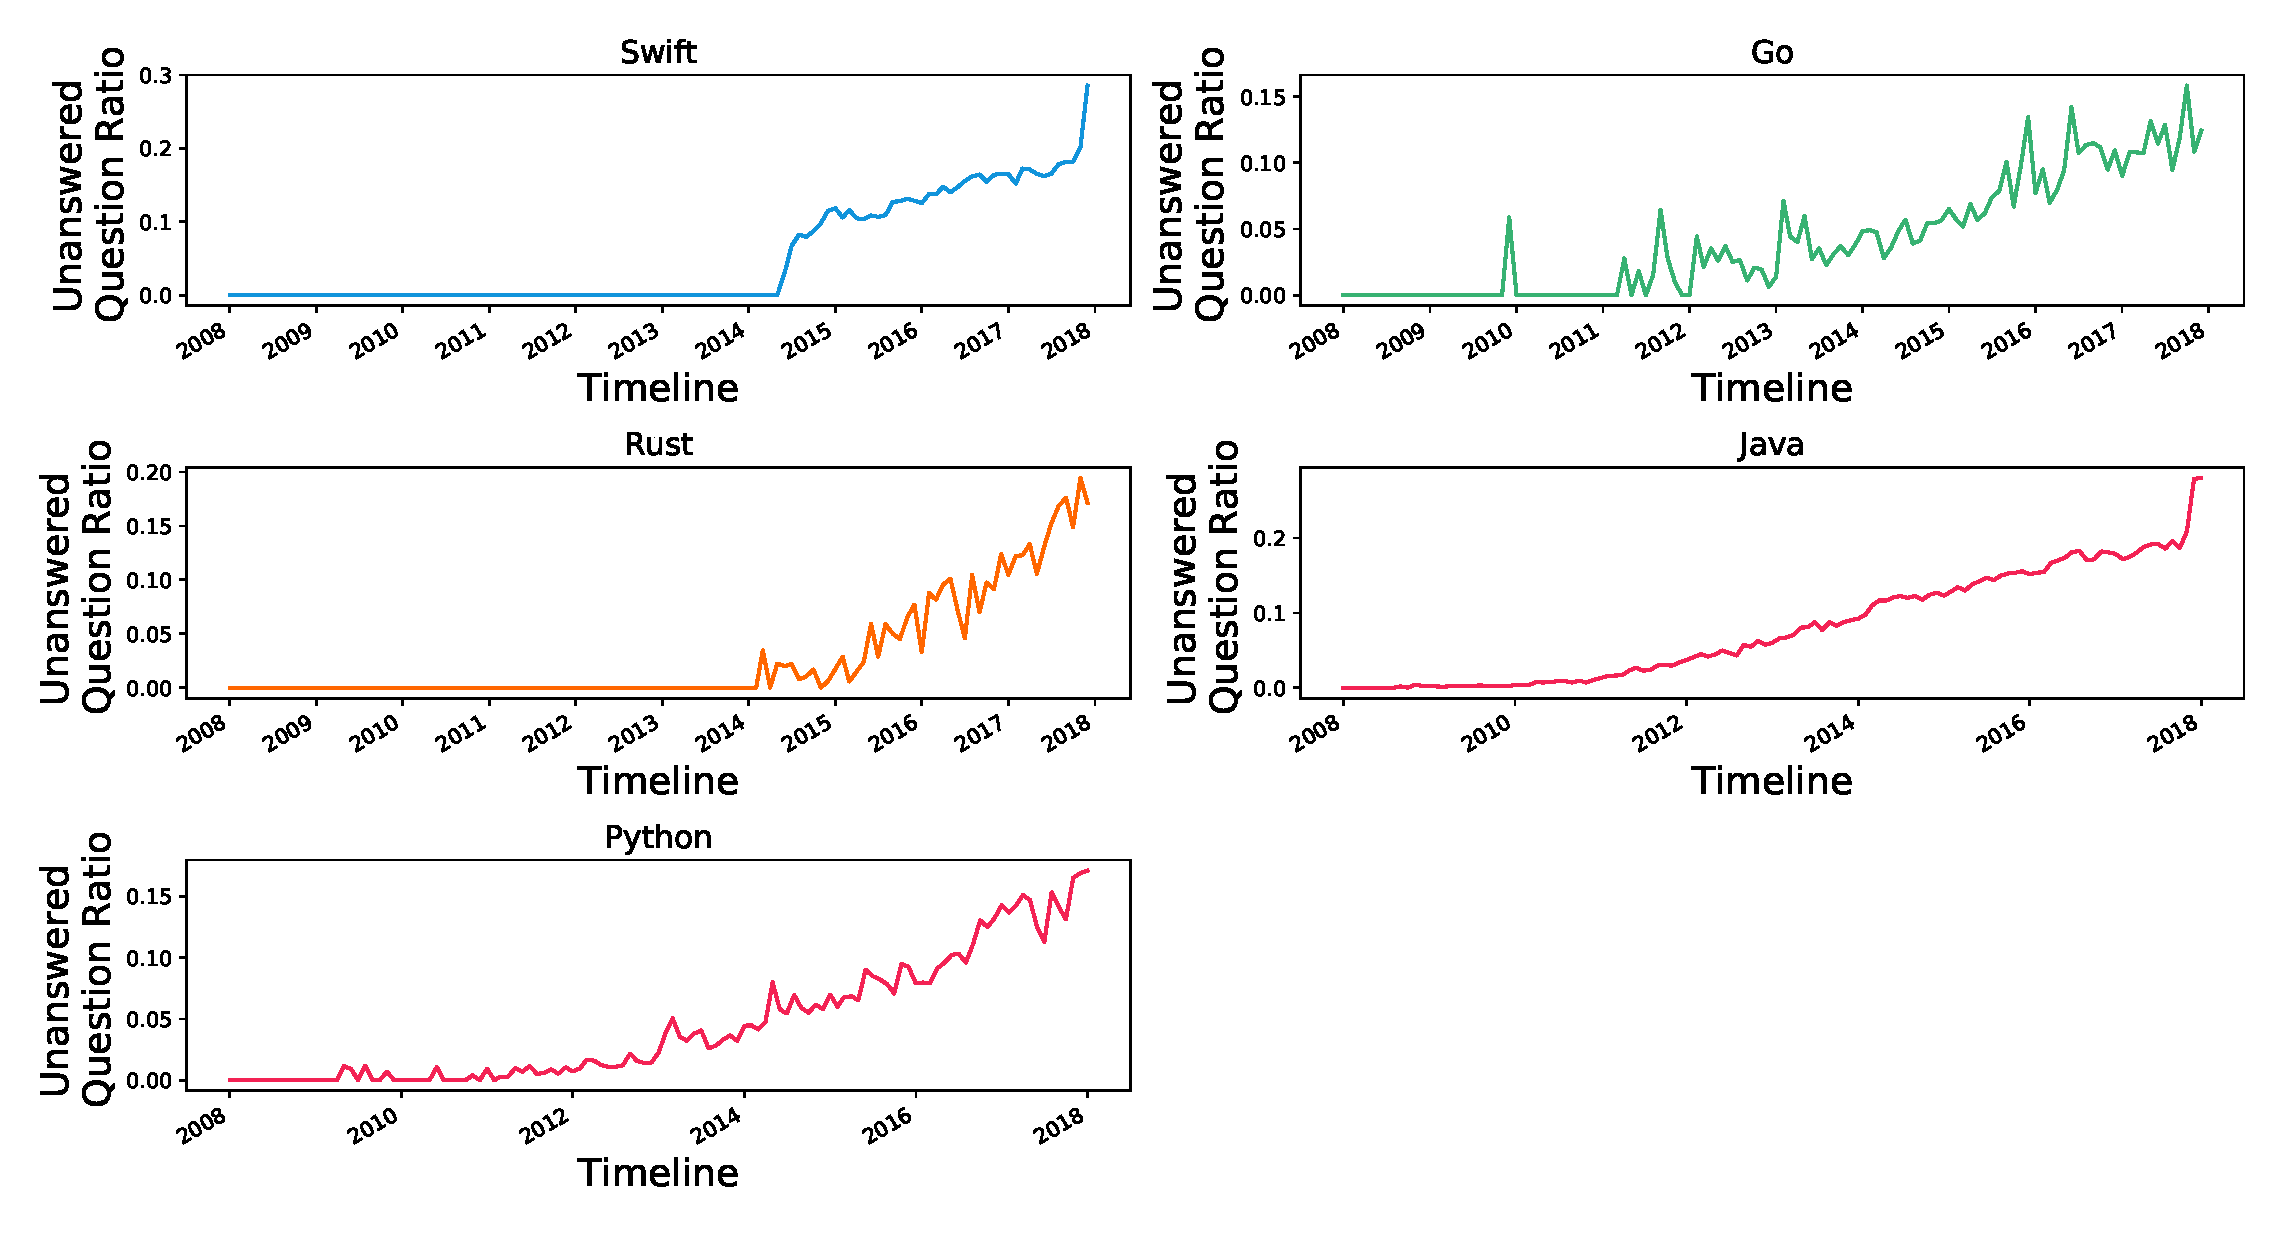
\includegraphics[scale=0.38]{figures/UnansweredQuestionRatio.eps}
\caption{Unanswered-question ratio in Stack Overflow}
\label{fig:Unanswered-question ratio}
\end{figure}


Figure~\ref{fig:Unanswered-question ratio} represents the contrariwise scenery of our assumption. As the day goes by, the unanswered question ratio increases. In one sense, we can say that the answer pattern for new languages and matured languages are the same as in both cases the unanswered question ration increases. However, we can observe two interesting phenomena from these results. First, the change ratio is smoother for matured language while it is notched for new languages except Swift. The reason for the jagged curve may be the absence of active expert developers. Inactive expert developers can change the ratio of the unanswered question by being active for a short time. That is why the curve for Go and Rust are jagged. Being the direct successor of Objective-C, Swift language has avoided this phenomenon. Second, Swift language starts its rise from a certain level which is caused by topic and question inheritance from Objective-C.

To compare growth, we plot the median time to get the first answer and the accepted answer of new languages and one matured language(in this case Java).
\begin{figure}[htbp]
\begin{subfigure}{0.6\textwidth}
\centering
\hspace{-3cm}
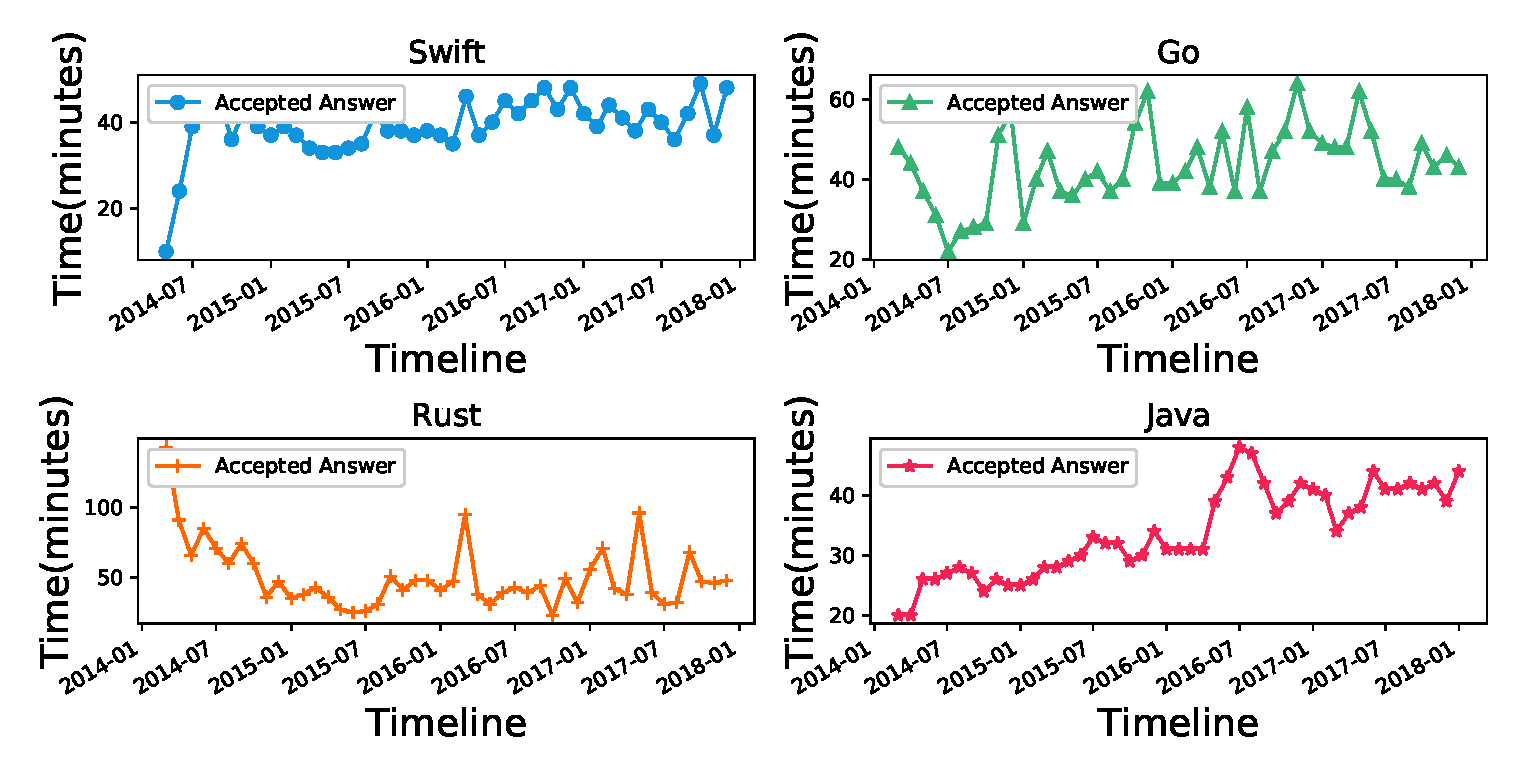
\includegraphics[scale=0.38]{figures/AcceptedAnswerInterval.eps}
\caption{\textbf{Accepted answer}}
\label{fig:Accepted Answer interval}
\end{subfigure}
\begin{subfigure}{0.6\textwidth}
\centering
\hspace{-3cm}
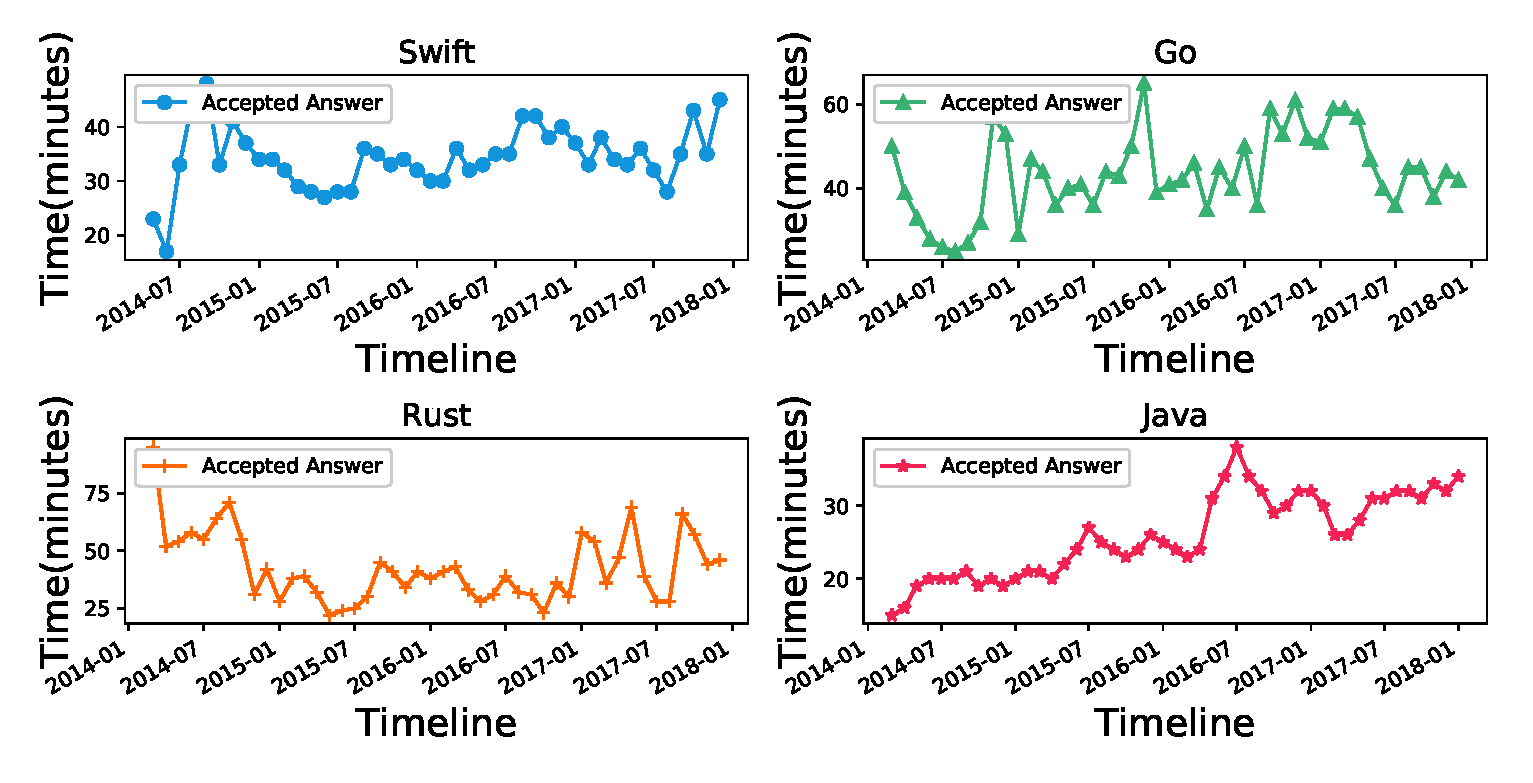
\includegraphics[scale=0.38]{figures/FirstAnswerInterval.eps}
\caption{\textbf{First answer}}
\label{fig:First Answer interval}
\end{subfigure}
\caption{Comparison of median answer interval  of languages in Stack Overflow}
\label{fig:Answer intervals}
\end{figure}
It is assumed that the interval of answers (first and accepted) will be decreased as the language evolves. However, Figure~\ref{fig:Answer intervals} proves that our assumption is wrong. The answer intervals of Java is increasing in the long run which may be caused by various reason. However, a common reason behind the long answer interval of  stack overflow questions is the inability of that question to attract an expert user to answer that question\citep{Asaduzzaman2013}.
Time to get an accepted answer indirectly represents the growth of developers' expertise. From Figure~\ref{fig:Accepted Answer interval}, it is prominent that Rust has comparatively longer accepted answer interval than the other two new languages. However, it is interesting that this is not true for the first answer interval. Go has longer first answer interval than Rust. Hence, we can say that the accepted answer interval of Rust is longer than Go but Go's first answer interval is longer than Rust. Longer accepted answer interval means the absence of expert developers. Thus, for the Go language, we can claim that Go developers receive the quality answer in the long run, but they have to wait a little longer as active support is absent. That means Stack overflow needs more \emph{active} Go developers and \emph{expert} Rust developers.


To strengthen our claim, we have performed Mann-Whitney U test for accepted answer interval and first answer interval of new languages. The result is presented in Table~\ref{table:accepted-first u value}.
\iffalse
\begin{table}
\centering
%\resizebox{\textwidth}{!}
\caption{Mann-Whitney U test result for the comparison of accepted answer time and first answer time of Go and Rust language}
\label{table:accepted-first u value}
\end{table}
\fi



\begin{table}
\caption{Mann-Whitney U test result for the comparison of accepted answer time and first answer time of Go and Rust language}
\begin{tabular}{|l|c|c|c|}
\hline
\multirow{2}{*}{Test Subject}                                   & \multicolumn{2}{c|}{Language}                                     & \multicolumn{1}{l|}{\multirow{2}{*}{p value}} \\ \cline{2-3}
                                                                & \multicolumn{1}{l|}{Language 1} & \multicolumn{1}{l|}{Language 2} & \multicolumn{1}{l|}{}                         \\ \hline
\multirow{3}{*}{First Answer Interval}                          & Go                              & Swift                           &     0.158                                          \\ \cline{2-4} 
                                                                & Go                              & Rust                            &    \textless 0.01                                           \\ \cline{2-4} 
                                                                & Swift                           & Rust                            &      \textless 0.01                                         \\ \hline
\multicolumn{1}{|c|}{\multirow{3}{*}{Accepted Answer Interval}} & Go                              & Swift                           &        0.389                                       \\ \cline{2-4} 
\multicolumn{1}{|c|}{}                                          & Swift                           & Rust                            &         \textless 0.1                                      \\ \cline{2-4} 
\multicolumn{1}{|c|}{}                                          & Go                           & Rust                            &           \textless 0.01                                    \\ \hline
\end{tabular}

\label{table:accepted-first u value}
\end{table}


From the Table~\ref{table:accepted-first u value}, we can reject the null hypothesis for first answer interval and accepted answer interval of Go-Rust and Swift-Rust pair. It means that the difference between first answer interval and accepted answer interval of Rust-Go and Swift-Rust is statistically significant. It implies that our claim about the first and accepted answer intervals of Go and Rust is true.

\boxtext{\textbf{Finding 7:} In Stack Overflow, it takes significantly higher time to get the first answer in the evolving state than the matured state of a new language.}

\boxtext{\textbf{Finding 8:} In Stack Overflow, we found evidence that Go has comparatively less active community support and Rust has a small number of expert developers.}
